\documentclass{article}
\usepackage{geometry}
\geometry{top=.5in,left=.3in,right=.3in,bottom=.5in}

\usepackage{pdfpages}
\usepackage{physics}
\usepackage{amsthm}
\usepackage{lipsum}
\usepackage{amsmath}
\usepackage{amssymb}

\begin{document}
  \twocolumn
    \subsection*{General Facts}
      Suppose $\hat{A}$ is either Hermitan or unitary. Then  $\hat{A}$ admits a 
      spectral decomposition. That is 
      \[
         \hat{A} = \sum_i \lambda_i \ket{i}\bra{i}
      .\] 
      For some basis $\{\ket{i} \}$. For operators with continuious spectrum,
      this sum is replaced by an integral. 
      Hermitan operators have real eigenvalues and unitary operators 
      have eigenvalues which lie on the complex unit circle.
      If two operators $\hat{A}$ and  $\hat{B}$ commute, then it is possible 
      to find a basis  $\{\ket{i}\}$ where $ \ket{i}$ is a simultaneous eigenket
      of both $\hat{A}$ and  $\hat{B}$
      If $\hat{A}$ is Hermitan, then  $e^{-i \hat{A} \cdot a / \hbar}$
      is Unitary

      The projector from one basis $ \{\ket{a_i}\}$ to another basis 
      $\{\ket{b_i}\}$ is a unitary operator \[
        \hat{U} = \sum_i \ket{b_i}\bra{a_i}
      .\] 
        
    \[
      \hat{p} = - i \hbar \frac{\partial}{\partial\,x} \quad
      \hat{x} = x \quad
      \hat{U} = e^{-i \hat{H} t / \hbar}
    \]
    
    \[
      [\hat{p},\hat{x}^n] = -i \,n \hbar \hat{x}^{n-1} \quad
      [\hat{x},\hat{p}^n] = i\,n  \hbar \hat{p}^{n-1} \quad
    \]
    \[
      [\hat{x},F(\hat{p})] = i \hbar \frac{\partial F}{\partial p} \quad
      [\hat{p},F(\hat{x})] =-i \hbar \frac{\partial F}{\partial x}
    \] 
    For some operator \(\hat{O}\) in the Schrodinger picture,
    the corresponding operator in the Heisenberg picture is 
    \(\hat{U}^\dagger\, \hat{O} \, \hat{U}\). And time dependence 
    in the Schrodinger picture is carried by \(\hat{U}\).
    

    \[
      i \hbar \frac{\partial}{\partial t} \ket{\varphi} = \hat{H} \ket{\varphi} 
      \iff \frac{d \hat{A}}{dt} = \frac{1}{i \hbar}[\hat{A},\hat{H}] + 
      \frac{\partial \hat{A}}{\partial t} 
    \]

    \subsection*{Two State Systems}
      \[
      \sigma_x = \begin{pmatrix} 0 & 1 \\ 1 & 0 \end{pmatrix} \quad
      \sigma_y = \begin{pmatrix} 0 & -i \\ i & 0 \end{pmatrix} \quad
      \sigma_z = \begin{pmatrix} 1 & 0 \\ 0 & -1 \end{pmatrix}
    \]

      \[ 
      [\sigma_i,\sigma_j] = \delta_{a b}I + i \epsilon_{ijk}\,\,\sigma_k \quad
      S_i = \frac{\hbar}{2}\sigma_i 
    \]
    The arbitrary 2--state Hamiltonian can be expressed as a linear combination
    of the $\sigma$ matrices and the identity matrix. This is sometimes written
    as an inner product as below.
    \[
      \hat{H} = A \bullet S + c\,\mathbb{I}
    .\] 

    For a charge in a magnetic field, with components $B_x$, $B_y$, and $B_z$
    the Hamiltonian is  \[
      \hat{H} =\frac{\hbar}{2} 
      \begin{pmatrix}
        B_z & B_x - i B_y \\ 
        B_x + i B_y  & - B_z
      \end{pmatrix}
    .\] 


      \[
      \ket{\uparrow} =
      \begin{pmatrix}
        1 \\ 
        0
      \end{pmatrix}
      \quad \lambda_\uparrow = \frac{\hbar}{2} \qquad
      \ket{\downarrow} = 
      \begin{pmatrix}
        0 \\ 
        1
      \end{pmatrix} \quad
      \lambda_\downarrow = -\frac{\hbar}{2}
      .\] 
      \[
      \ket{+} = \frac{1}{\sqrt 2}
      \begin{pmatrix}
        1 \\ 
        1
      \end{pmatrix}
      \quad \lambda_+= \frac{\hbar}{2} \qquad
    \]
    \[
      \ket{-} = \frac{1}{\sqrt 2}
      \begin{pmatrix}
        1 \\ 
        -1
      \end{pmatrix} \quad
      \lambda_-= -\frac{\hbar}{2}
      .\] 
      




    \subsection*{Harmonic Oscillator} 
      \[
        V = \frac{1}{2} m \omega^2 x^2 \quad 
        \hat{a} = \sqrt{\frac{m \omega}{2 \hbar}}( \hat{x} + \frac{i}{m \omega}\hat{p})
      \]

      \[
        \hat{x} = \sqrt{\frac{\hbar}{2 m \omega}}(\hat{a}^\dagger + \hat{a}) \quad
        \hat{p} = i \sqrt{\hbar m \omega /2 }(\hat{a}^\dagger - \hat{a}) \quad
        \hat{H} = \hbar \omega(\hat{a}^\dagger\hat{a} + \frac{1}{2})
      \]
      \[
      \hat{N} = \hat{a}^\dagger \hat{a} \quad \hat{N} \ket{n} = n \ket{n} 
      .\]  
      \[
        [\hat{a},\hat{a}^\dagger] = 1 \quad
        \hat{a}^\dagger \ket{n} = \sqrt{n + 1} \ket{n+1} \quad
        \hat{a} \ket{n} = \sqrt{n}\ket{n-1}
      \]
  
      \[
        \hat{a}(t) = e^{-i \omega t}\hat{a}(0) \quad 
        \hat{p}(t) = - m \omega \hat{x}(0) \sin(\omega t) + \hat{p}(0) \cos(\omega t) 
      \]
    
      \[
        \hat{x}(t) = \hat{x}(0) \cos(\omega t) + \frac{\hat{p}(0)}{m \omega }\sin(\omega t)
      \]
    \subsection*{Parity and Symmetry}    
      The parity operator $\hat{P}$ is defined by its action on the position 
      operator, that is  $\hat{P}^\dagger \hat{x} \hat{P} = - \hat{x}$. Therefore
      it is also the case that \[
        \hat{P}\ket{x} = \ket{-x}  \quad \hat{P}\ket{p} = \ket{-p}
      .\] 
      From this, we can see that $\hat{P}^{\dagger}\hat{p}\hat{P} = -\hat{p}$ 
      An operator $\hat{O}$ has is a symmetry of $\hat{A}$ if 
      $[\hat{A},\hat{O}]=0$ and $\hat{O}$ preserves probabilities in general.
      Symmetries must be unitary.
      In the position basis, even functions are of even parity and odd 
      functions are of odd parity.
      
      If $\hat{H}$ is a Hamiltonian which has a potential with periodicity  $a$
      Then 
      \[
        \hat{\tau}(a) = e^{-\frac{i a \cdot \hat{p} }{\hbar}}
      .\]  
      Is a symmetry of the Hamiltonian 
      If $\hat{U}$ is a symmetry of some hamiltonian generated by  $\hat{Q}$
      Then  $[\hat{H},\hat{Q}] = 0 \implies \frac{d\hat{Q}}{dt} = 0$

    \subsection*{Translation and Bloch's Theorem}
      \[
        \hat{\tau}(a) \ket{x} = \ket{x + a}
      .\]  
      Momentum is the generator of translation. 
      If $\hat{H}$ is a Hamiltonian with potential that has period $a$
      and some (potentially infinite) number of disconnected wells, we may 
      label the eigenstates of  $\hat H$ as  $ \ket{n,E}$ where  $n$ 
      corresponds to the localization of the state, and  $E$ is the eigenvalue
      of  $\hat H $ corresponding to  $\ket{n,E}$. We can find a linear 
      combination of these states, $\ket{\theta,E} = \sum_n e^{i n \theta}\ket{n,E}$
      \[
        \hat{\tau}(a) \ket{\theta,E} = e^{-i\theta}\ket{\theta,E}
      .\] 
      When the number of wells is finite, this quantizes $\theta$
      The \textbf{Tight Binding Approximation} is the assumption that 
      \[
        \bra{n,E}\hat{H}\ket{n+m,E}=0 \,\,:\,\, |m| > 1
      .\] 
     Bloch's Theorem says that, in such a system, \[
       \bra{x}\ket{\theta}= e^{i \theta x /a}u_k(x) \,\,:\,\, u_k(x + a) = u_k(x)
     .\]  
     The \textbf{Brillioun Zone} associated with a potential is 
     The set of physically distinct values of $k$ for which energy is defined 
     in terms of  $k$.

  \subsection*{Scattering and Wave mechanics}
    \[
      V(x) = 
      \begin{cases}
        0 & x < a_1 \\
        V(x) & a_1 \leq x \leq a_2 \\
        0 & x > a_2
      \end{cases} 
      \implies 
    \]
    \[
      \varphi(x) = 
      \begin{cases}
        A e^{i k x} + B e^{-i k x} & x < a_1 \\
        garbage & a_1 \leq x \leq a_2 \\
        F e^{i k x} + G e^{-i k x} & x > a_2
      \end{cases}
    .\] 
    \[
    T = \left|\frac{F}{A}\right|^2 \quad R = \left|\frac{B}{A}\right|^2
    .\]    
   The $S$ matrix is defined by the relation.
   \[
   \begin{pmatrix}
     F \\
     B
   \end{pmatrix}
   = 
   \begin{pmatrix}
     S_{11} & S_{12} \\
     S_{21} & S_{22} 
   \end{pmatrix}
   \begin{pmatrix}
     A \\
     G
   \end{pmatrix}
   .\] 
   Which is unitary.


  \subsection*{The WKB Approximation}
    \[
    \kappa(x) = \sqrt{\frac{2m}{\hbar^2}(V(x) - E)} \quad
    k(x) = \sqrt{\frac{2m}{\hbar^2} E - V(x)}
    .\]    
    \[
      \varphi(x) = 
      \begin{cases}
        \frac{1}{\sqrt{k(x)}} \exp[\pm i \int^x k(x)\,\,dx ]& E > V(x) \\
        \frac{1}{\sqrt{\kappa(x)}} \exp[\pm \int^x \kappa(x) \,\,dx] & E < V(x)
      \end{cases}
    .\] 
    If $\frac{d V}{dx}|_{x=a} > 0$ 
    \[
      \frac{A}{\sqrt{\kappa(x)}}\exp\left[ -\int_a^x \kappa(x')\,dx' \right] +
      \frac{B}{\sqrt{\kappa(x)}}\exp\left[\int_a^x \kappa(x)\,\,dx'\right] =
    \] 
    \[
      \frac{2A}{\sqrt{k(x)}}\cos\left[\int_x^a k(x')\,dx' - \frac{\pi}{4} \right] -
      \frac{B}{\sqrt{k(x)}}\sin\left[\int_x^a k(x')\,dx' - \frac{\pi}{4}\right]
    .\] 
    If the derivative at $a$ flips sign, you just flip all limits of inegration
    to get the correct expression.
    \subsubsection*{Trig Identities for WKB}
      \[
        \sin(\theta \pm \frac{ \pi}{2}) = \pm\cos(\theta) \quad
        \cos(\theta \pm \frac{\pi}{2}) = \mp\sin(\theta)
      .\] 
      \[
        \sin(\alpha \pm \beta) = \sin(\alpha)\cos(\beta) \pm \cos(\alpha)\sin(\beta)
      .\] 
      \[
        \cos(\alpha \pm \beta) = \cos(\alpha)\cos(\beta) \mp \sin(\alpha) \sin(\beta)
      .\] 
      \[
        2\cos(\theta)\cos(\varphi) = \cos(\theta - \varphi) + \cos(\theta + \varphi)
      .\] 
       \[
         2\sin(\theta)\sin(\varphi) = \cos(\theta - \varphi) - \cos(\theta + \varphi)
      .\] 
      \[
        2 \sin(\theta)\cos(\varphi) = \sin(\theta + \varphi) + \sin(\theta - \varphi)
      .\] 
      \[
        2\sin(\theta)\sin(\varphi) = \sin(\theta + \varphi) - \sin(\theta - \varphi)
      .\] 

  \subsubsection*{Spherically Symmetric Potentials}
    If a particle is subjected to a purely radial potential, its wavefunction
    is given by $\varphi_{nlm} = R_{nl}Y_l^m$ where  $R_{lm}$ satisfies.
    \[
      \frac{d^2 R_{nl}}{d\rho^2} + \frac{2}{\rho}\frac{d R_{nl}}{d\rho} + 
      (1 - \frac{l (l+1)}{\rho^2})R_{nl} = 0 \quad \rho = r\sqrt{2m(E-V)/\hbar^2} 
    .\] 
    \[
      u_{nl} = r R_{nl} \quad \frac{-\hbar^2}{2m}\frac{d^2}{dr^2}u_{nl} + 
      \left(\frac{l(l+1)\hbar^2}{2mr^2}+V\right)u_{nl} = E\, u_{nl}
    .\] 
  \section*{Propagators and Path integrals}
    The propogator of a particle subject to a Hamiltonian $\hat H $ is given by 
     \[
       K(x',t;x,t_0) = \bra{x'} e^{- i \hat{H}(t-t_0)/\hbar} \ket{x} = 
       \sum_a \bra{x'}\ket{a}\bra{a}\ket{x}e^{-i E_a (t - t_0)/\hbar}
    .\] 
    And note further that such propagators compose as 
    \[
      K(x'',t'';x,t_0) = \int K(x'',t'';x',t') \times K(x',t';x,t_0)d^3 x'
    .\] 
    Now, let the action of the classical analogue of a quantum system be given by 
    \[
      S = \int_{t_1}^{t_N} dt \mathcal{L}(x,\dot x) \text{ and }  \delta t = \frac{t_N - t_{1}}{N - 1}
    .\] 
    Then, the path integral for 
    \[
      \lim_{\delta t \rightarrow 0} \bra{x_N,t_N}\ket{x_1,t_1} = 
      \int_{x_1}^{x_N} \mathcal{D}[x(t)] e^{i S(x,\dot x) / \hbar}
    \]
    where \[
      \int_{x_1}^{x_N}\mathcal{D}[x(t)] = \lim_{N \rightarrow \infty}
      (\frac{m}{2 \pi i \hbar  \,\delta t})^{(N-1)/2} 
      \int dx_{N-1} \int dx_{N-2} \dots \int dx_1 
    .\] 

  \section*{Gauge Symmetry}
    Classically, electromagnetic fields are invariant under a gauge transformation
    of the form $\phi \rightarrow \phi + \lambda$ and  $A \rightarrow A + \nabla \Lambda$. 
    Where $A$ is a vector potential (I neglect to place vector arrows). 
    The Hamiltonian for a charged particle subject to such a potential is 
     \[
       \hat H = \frac{1}{2m} \hat \Pi^2 + e \phi \text{ with } \hat\Pi = p - \frac{e}{c}A
    .\] 
    In the Heisenberg picture, we have that \[
      m \frac{d\hat{x}}{d t} = \hat{\Pi} \text{ and } [\hat{\Pi}_i,\hat{\Pi}_j] = 
      \frac{i \hbar e}{c }\epsilon_{ijk} B_k
    .\] 
    Furthermore, we see that our wavefunction transforms as \[
      \ket{\varphi} \rightarrow e^{i e \Lambda / \hbar c}\ket{\varphi}
    .\] 
    Note that the kinematical momentum $\hat \Pi $ is invariant under gauge
    transformations by construction. 

  \section*{Angular Momentum}
    We denote the angular momentum operator as $\hat J$, and the components of this
    operator as  $\hat J _i $.
    Angular momentum is the generator of rotations; 
    \[
      \hat{R}(x_i,\theta) = \exp[- i \hat J _i \theta / \hbar]
    .\] 
    \[
      \begin{split}
      \hat{J}_\pm = \hat{J}_x \pm i \hat{J}_y \quad
      [\hat J _i, \hat J _j] = i \hbar \epsilon_{ijk} J_k \quad \\
      [\hat J _z, \hat{J}_\pm] = \pm \hbar \hat{J}_\pm \quad
      [\hat J _+, \hat J _-] = 2\hbar J_z
    \end{split}
    .\]\[
    (\hat{J}^2, \hat{J}_z)\ket{j,m} = (\hbar^2j(j+1),\hbar m)\ket{j,m} \quad
    \]\[
    \hat{J}_{\pm} \ket{j,m} = \sqrt{(j\mp m)(j \pm m + 1)}\ket{j,m\pm 1} \quad
    \hat{J}_z = -i\hbar\frac{\partial}{\partial \phi}
    .\]   
    Suppose now that we have two different particles with angular momentum 
    operators $\hat J _1$ and $\hat J _2$ so that  $\hat J = \hat J _1 +\hat J_2$.
    Then  $2 J_1 \bullet J_2 = J^2 - J_2^2 - J_1^2$.

    \section*{Clebsch Gordan Coefficients}
      The Clebsch--Gordan coefficients are change of basis matrix elements 
      to transform between two CSCO's which are 
      $\{\hat J ^2, \hat J _z \hat J _1 ^2 , \hat J _2 ^2\}$ and 
      $\{\hat J _1^2 , \hat J _2^2 \hat J _{1z} , \hat J _{2z} \}$.
      A table of coefficients has been appended to this document. 
      The components are represented as the overlap of an eigenstate of one 
      CSCO with an eigenstate of the other CSCO. $\bra{j_1,j_2,m_1,m_2}\ket{j_1,j_2,j,m}$


    \section*{Tensor Products and Direct Sums}
    Let $A$ and  $B$ be matrices with matrix elements $a_{ij}$ and  $b_{ij}$.
    Let us define  $\vec a$ and  $ \vec b$ as vectors which can be operated on 
    by  $A$ and $B$ respectively. In block form, 
    \[
    A \oplus B = 
    \begin{pmatrix}
      A & 0 \\
      0 & B
    \end{pmatrix}
    \quad
    \vec{a} \oplus \vec{b} = 
    \begin{pmatrix}
      \vec a \\
      \vec b
    \end{pmatrix}
    \quad 
    (A_1 \oplus A_2)(B_1 \oplus B_2) = A_1 B_1 \oplus A_2 B_2
    \] 
    Tensor products have similar arithmetic rules. 
    \[
    A \otimes B = 
    \begin{pmatrix}
      A_{11} B  & A_{12}B & A_{13} B & \dots \\
      A_{21} B & A_{22} B & A_{23} B & \dots \\
      A_{31} B & A_{32} B & A_{33} B & \dots \\
      \vdots & \vdots  & \vdots  & \ddots
      
    \end{pmatrix}
    .\] 

  \section*{Tensors and More Angular Momentum}
    From a nasty and obscure derivation using the Wigner D matrix, 
    we have the identity that  \[
      \begin{split}
        \int d\Omega Y_{lm}^* Y_{l_1 m_1} Y_{l_2 m_2} = 
      \sqrt{\frac{(2l_1 +1)(2l_2 +1)}{4 \pi (2 l + 1)}} 
      \bra{l_1,l_2;00}\ket{l_1,l_2;l_0} \times \\
      \bra{l_1,l_2;m_1,m_2}\ket{l_1,l_2;l,m}
      \end{split}
    .\] 
   
    If $T_q^k$ is a spherical tensor of rank  $k$, then 
     \[
    \bra{\alpha',l',m'} T_q^k \ket{\alpha, l, m} = 0 
    \text{ unless } m' = m + q \text{ and } |j-k| \leq j' \leq j+k
    .\] 
    Cartesian vector operators satisfy the commutation relation
    \[
      [V_i, J_j] = i \hbar \epsilon_{ijk} V_k \text{ so }
      V^1_{\pm 1} = \mp \frac{1}{\sqrt 2} (V_x \pm i V_y) \quad V_0^1 = V_z
    .\] 
    Spherical tensors obey the equations (which suffices as a definition)
    \[
      [\hat{J}_z , T_q^k] = \hbar q T_q^k \quad 
      [\hat{J}_\pm , T_q^k ] = \hbar \sqrt{(k\mp q)(k\pm q + 1)}T_{q\pm 1}^k
    \] 
    Any rank $2$ Cartesian tensor can be decomposed as 
    $T_{ij} = E \delta_{ij} + A_{ij} + S_{ij} $ where  \[
    \begin{split}
      E = \frac{1}{3} \sum_i T_{ii} \quad A_{ij} = \frac{1}{2}(T_{ij} - T_{ji}) \\
      S_{ij} = \frac{1}{2}(T_{ij} + T_{ji}) - \frac{1}{3} \delta_{ij} \sum_k T_{kk} 
    \end{split}
    \] 
    Then, the components of the spherical tensors are 
    \[
      \begin{split}
      T_0^0 = E ,\quad T_0^1 = A_{xy} ,\quad 
      T_{\pm_1}^1 = \mp \frac{1}{\sqrt 2} (A_{yz} \pm i A_{zx}) ,\quad
      T_0^2 = \sqrt{3/2} S_{zz}, \\
      T_{\pm 1}^2 = \mp (S_zx \pm i S_zy) ,\quad 
      T_{\pm 2}^2 = \frac{1}{2}(S_{xx} - S_{yy} \pm 2 i S_{xy})
      \end{split}
    \] 
    If $X_{q_1}^{k_1}$ and $Z_{q_2}^{k_2}$ are spherical tensors then 
    \[
      T_q^k = \sum_{q_1, q_2} \bra{k_1,k_2;q_1,q_2}\ket{k_1,k_2;k,q}X^{k_1}_{q_1}Z_{q_2}^{k_2}
    .\] 
    
    is also a spherical tensor. This is inverted by 
    \[
      X_{q_1}^{k_1}Z_{q_2}^{k_2} = \sum_{k=|k_1-k_2|}^{k_1+k_2} \sum_{q = -k}^k
      \bra{k_1,k_2;k,q}\ket{k_1,k_2;q_1,q_2}
    .\] 
    Explicitly, for combining two rank one spherical tensors, $U$ and  $V$ then,
     \[
    \begin{split}
      T^2_{\pm 2} = U_{\pm 1} V_{\pm 1} \quad T^2_{\pm 1} = \frac{1}{\sqrt 2}
      (U_{\pm 1}V_0  + U_0 V_{\pm 1}) \\
      T^2_0 = \frac{1}{\sqrt 6 } (U_1 V_{-1} + 2 U_0 V_0 + U_{-1}V_1)
    \end{split}
    .\] 

    \subsubsection*{The Wigner--Eckhart Theorem and Corollaries}
      The Wigner--Eckhart Theorem says that, if $T_q^k$ is a spherical tensor,
      \[
        \bra{\alpha',l\,m}T_q^k\ket{\alpha ,l,m} = \frac{1}{\sqrt{2 j' + 1}}
      \bra{j,k;m,q}\ket{j,k;j',m'}\bra{\alpha',j'}|T^k|\ket{\alpha,j}
      .\] 
      The Wigner--3j symbols are written as 
      \[
      \begin{pmatrix}
        j_1 & j_2 & j_3 \\
        m_1 & m_2 & m_3
      \end{pmatrix}
      .\] 
      \[
        \begin{split}
          \bra{j_1,j_2;m_1,m_2}\ket{j_1,j_2;j,m} = (-1)^{j_1+j_2+j} \sqrt{2j+1}
          \begin{pmatrix}
            j_2 & j_1 & j \\
            m_1 & m_2 & -m
          \end{pmatrix} \\
          \begin{pmatrix}
            j_1 & j_2 & j \\
            m_1 & m_2 & m 
          \end{pmatrix} = 
          \begin{pmatrix}
            j & j_1 & j_2 \\
            m & m_1 & m_2 
          \end{pmatrix} = (-1)^{j_1 + j_2 + j} 
          \begin{pmatrix}
            j_2 & j_1 &j \\
            m_2 & m_1 & m
          \end{pmatrix} \\
          \begin{pmatrix}
            j_1 & j_2 & j \\
            -m_1 & -m_2 & -m 
          \end{pmatrix} = (-1)^{j_1 + j_2 + j}
          \begin{pmatrix}
            j_1 & j_2 & j \\
            m_1 & m_2 & m
          \end{pmatrix} \\
          (-1)^{1 - j - m}\frac{m}{\sqrt{j(j+1)(2j+1)}} = 
          \begin{pmatrix}
            j & 1 & j \\
            m & 0 & -m
          \end{pmatrix}
        \end{split}
      .\] 
      The Projection theorem states that if $J_q$ is an angular momentum 
      operator  and  $V_q$ is a rank one spherical tensor, 
      \[
        \bra{\alpha',j,m'}V_q\ket{\alpha,j,m} = 
        \frac{\bra{\alpha',j,m'}J\bullet V\ket{\alpha,j,m}}{\hbar^2 j(j+1)}
        \bra{j,m'}J_q\ket{j,m}
      .\] 
      

    % start with CG coeffs Nov 13 lecture, and go through wigner D--matrix
    % and tensor stuff and the wigner--eckhart theorem. Try to understand 
    % wtf he means by the tensor product/ direct sum equivalence
   \onecolumn
   \begin{figure}
      \centering 
      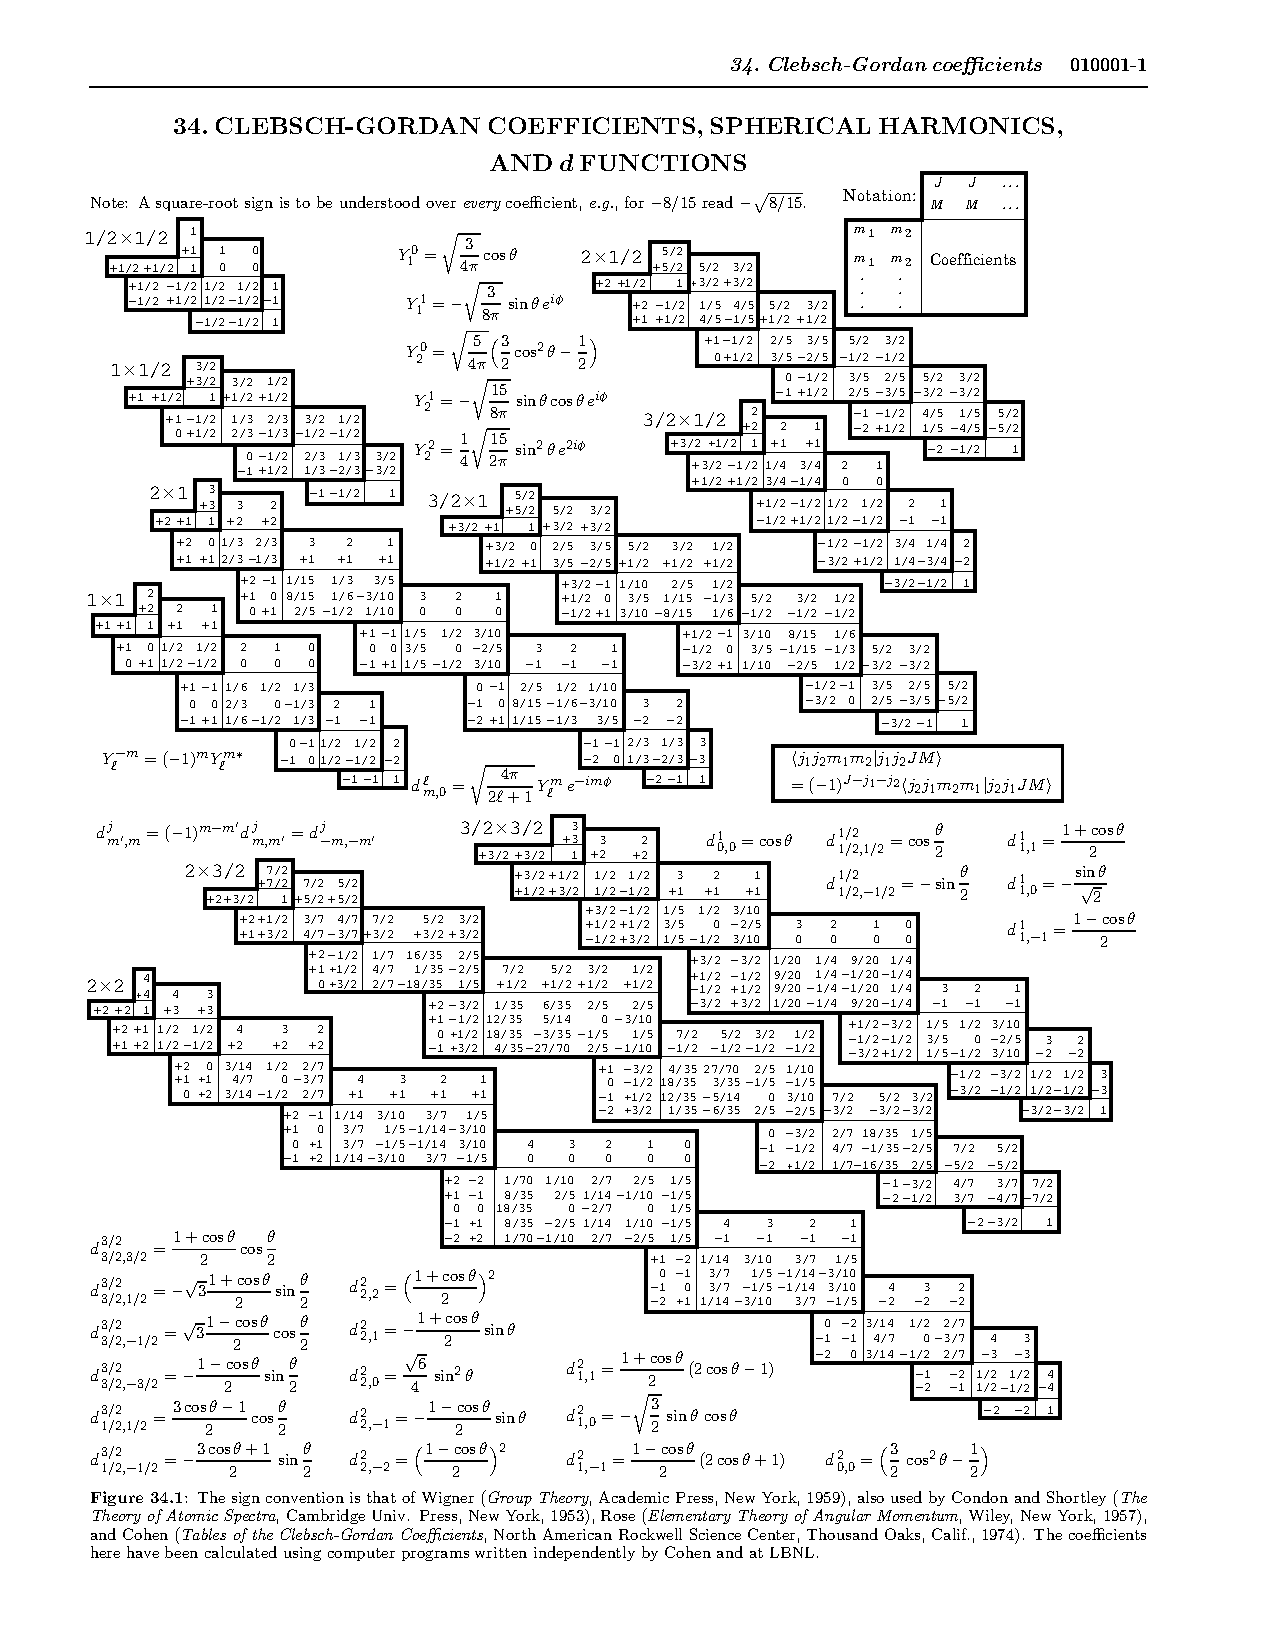
\includegraphics{./clebrpp.pdf}
   \end{figure} 









\end{document}
